\documentclass[11pt]{article}

\usepackage{amsmath}
\usepackage{amssymb}
\usepackage{bm}
\usepackage{caption}
\usepackage{CJKutf8}
\usepackage{color}
\usepackage{enumitem}
\usepackage{float}
\usepackage{flowchart}
\usepackage{graphicx}
\usepackage{geometry}
\usepackage{indentfirst}
\usepackage{listings}
\usepackage{mathdots}
\usepackage{mathpazo}
\usepackage{pstricks-add}
\usepackage{pst-blur}
\usepackage{subcaption}
\usepackage{tikz}
\usepackage{wasysym}
\usepackage{xcolor}
\usepackage[BoldFont,SlantFont,CJKsetspaces,CJKchecksingle]{xeCJK}

\allowdisplaybreaks
\definecolor{Blue}{rgb}{1.,0.75,0.8}
\definecolor{mygray}{rgb}{0.5,0.5,0.5}
\definecolor{mygreen}{rgb}{0,0.6,0}
\definecolor{mymauve}{rgb}{0.58,0,0.82}
\pagestyle{empty}
\parindent 2em   %段首缩进
\setlength{\parindent}{2em}
\setCJKmainfont[BoldFont=SimHei]{SimSun}
\setCJKmonofont{SimSun}% 设置缺省中文字体
\usetikzlibrary{arrows, automata, calc, shapes}

\newcommand{\hytt}[1]{\texttt{\hyphenchar\font=\defaulthyphenchar #1}}
\hyphenation{read-Sym-bol re-ad-Space-Tab-New-line str-Tab}

%\footnotesize
\lstset{ %
  backgroundcolor=\color{white},   % choose the background color; you must add \usepackage{color} or \usepackage{xcolor}
  basicstyle=\ttfamily,            % the size of the fonts that are used for the code
  breakatwhitespace=false,         % sets if automatic breaks should only happen at whitespace
  breaklines=true,                 % sets automatic line breaking
  captionpos=b,                    % sets the caption-position to bottom
  commentstyle=\ttfamily\color{mygreen},    
                                   % comment style
  deletekeywords={},               % if you want to delete keywords from the given language
  escapeinside={},                 % if you want to add LaTeX within your code
  extendedchars=true,              % lets you use non-ASCII characters; for 8-bits encodings only, does not work with UTF-8
  frame=single,                    % adds a frame around the code
  keepspaces=true,                 % keeps spaces in text, useful for keeping indentation of code (possibly needs columns=flexible)
  keywordstyle=\color{blue},       % keyword style
  language={[x86masm]Assembler},                    % the language of the code
  morekeywords={},                 % if you want to add more keywords to the set
  numbers=left,                    % where to put the line-numbers; possible values are (none, left, right)
  numbersep=5pt,                   % how far the line-numbers are from the code
  numberstyle=\tiny\color{mygray}, % the style that is used for the line-numbers
  rulecolor=\color{black},         % if not set, the frame-color may be changed on line-breaks within not-black text (e.g. comments (green here))
  showspaces=false,                % show spaces everywhere adding particular underscores; it overrides 'showstringspaces'
  showstringspaces=false,          % underline spaces within strings only
  showtabs=false,                  % show tabs within strings adding particular underscores
  stepnumber=1,                    % the step between two line-numbers. If it's 1, each line will be numbered
  stringstyle=\color{mymauve},     % string literal style
  tabsize=2,                       % sets default tabsize to 2 spaces
  title=\lstname,                   % show the filename of files included with \lstinputlisting; also try caption instead of title
  texcl=true
}

\begin{document}
% \begin{CJK}{UTF8}{gkai}
\title{接口技术课程设计报告\\多功能时钟的设计与实现}

\author{计算机1202 张艺瀚\\学号:20123852}
\maketitle

\section{目的与功能}
设计实现一个多功能时钟.8个LED灯用BCD码形式显示当前小时(0-23),每逢24小时重置为0时.每逢整点则播放一段音乐(《送别》).

\section{原理与过程}
8255的A口接门控开关,用于控制LED灯.B口接LED灯,用于以2位BCD码形式显示当前小时.

8253的通道0用于控制扬声器发声,CLK0接脉冲发生器的CLK2,CLK2为1.5MHz的时钟,GATE0接常有效,OUT0接扬声器的A.IN,用于发声.通道1和2对输入时钟连续分频,用于计时,CLK1接脉冲发生器的CLK4,CLK4为0.375MHz的时钟,GATE1接常有效,OUT1接CLK2作为通道2的输入时钟,再次分频,GATE2接常有效,OUT2接8259的IR0,用于整点时产生中断.

8253的通道1的输入时钟为0.375MHz,而每过1小时产生一次输出,从而可以算出其计数初值为
\[ \frac{0.375MHz}{\dfrac{1}{3600}Hz} = 1348920863 = 5066E61F \]
这个数太大了,所以我们用通道2对通道1的输出时钟再分一次频,这样,通道1和2的计数初值应为
\[ \sqrt{1348920863} = 36278 = 87F8 \]

每逢整点,就会产生中断,在中断服务程序中做2件事:将当前的小时计数+1,点亮LED灯对应位,以BCD码形式显示当前小时;调用music子程序播放音乐.


为了播放音乐,我编写了sound子程序,用于发出某一频率的声音,在music子程序中读乐谱,调用sound子程序播放每一个音,就形成了乐曲.

在sound子程序中,为了使8253控制扬声器发出某一频率的声音,需要为8253送计数初值,该计数初值由下面的公式得到
\[ \text{计数初值}=\frac{1.5MHz}{\text{待播放音符的频率}} \]

8255片选接CS0,A口,B口和控制口的地址分别为04a0,04a2和04a6;
8253片选接CS1,通道0,1和2以及控制口的地址分别为04b0,04b2,04b4,04b6;
8259片选接CS2,它的2个端口地址分别为04c0和04c2.
各芯片的数据线,地址线,读写线直接与8086CPU连接即可.

关于设计实现的其他细节,见程序清单中的注释.

\section{电路原理图}
多功能时钟的电路原理图如下(图~\ref{fig: circuit} ).数据总线有8位,用一条红线表示.
\begin{center}
\begin{figure}
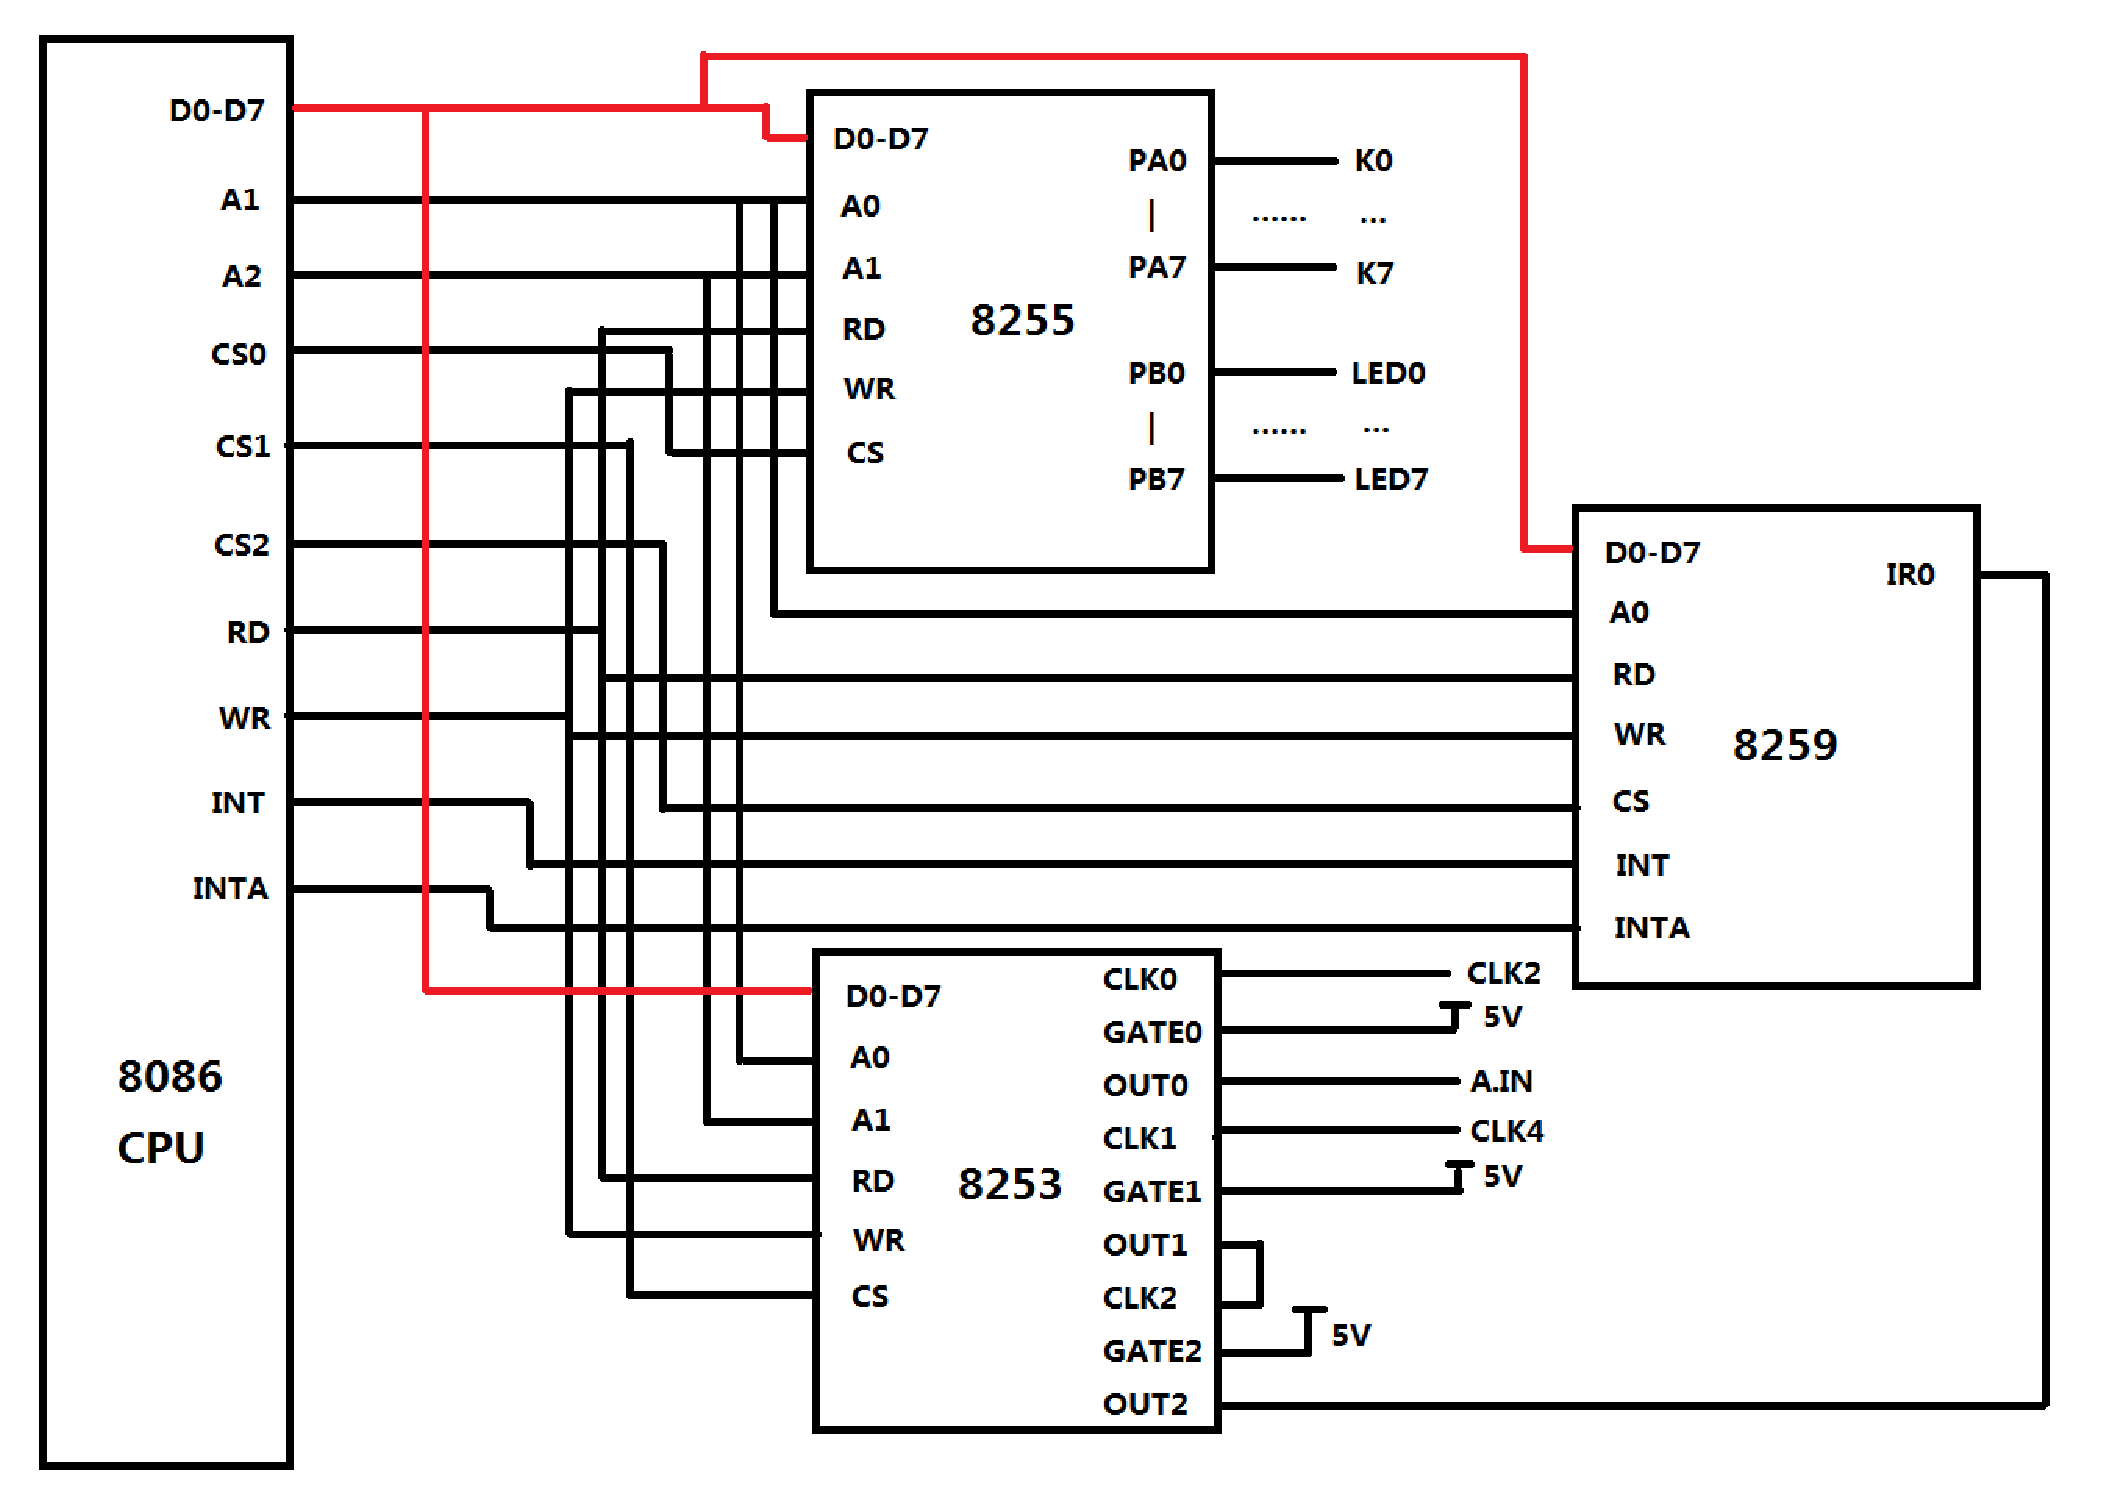
\includegraphics[width=\textwidth]{circuit.eps}
\caption{多功能时钟电路原理图}
\label{fig: circuit}
\end{figure}
\end{center}

\section{程序流程图}

程序流程图如图~\ref{fig: main},图~\ref{fig: flowchart},图~\ref{fig: music}.

% 流程图定义基本形状
\tikzstyle{startstop} = [rectangle, rounded corners, minimum width=3cm, minimum height=1cm,text centered, draw=black, fill=red!30]
\tikzstyle{io} = [trapezium, trapezium left angle=70, trapezium right angle=110, minimum width=3cm, minimum height=1cm, text centered, draw=black, fill=blue!30]
\tikzstyle{operation} = [rectangle, minimum width=3cm, minimum height=1cm, text centered, draw=black, fill=orange!30]
\tikzstyle{judge} = [diamond, minimum width=3cm, minimum height=1cm, text centered, draw=black, fill=green!30]
\tikzstyle{arrow} = [thick,->,>=stealth]

\begin{figure}
\centering
\begin{tikzpicture}[node distance=2cm]
%定义流程图具体形状
\node (start) [startstop] at(0,0)		{开始};
\node (a) [operation] at(0,-2) 			{关中断};
\node (b) [operation] at(0,-4)			{设置中断向量表};
\node (c) [operation] at(0,-6)			{8259初始化};
\node (d) [operation] at(0,-8)			{8255初始化};
\node (e) [operation] at(0,-10)			{8253初始化};

\node (f) [operation] at(4,-8) 			{开中断};
\node (g) [operation] at(4,-6)			{读8255的A口};
\node (h) [operation] at(4,-4)			{设置al为当前小时};
\node (i) [operation] at(4,-2)			{al送8255的B口};

%连接具体形状
\draw [arrow](start) -- (a);
\draw [arrow](a) -- (b);
\draw [arrow](b) -- (c);
\draw [arrow](c) -- (d);
\draw [arrow](d) -- (e);
%\draw [arrow]( ) -- node[anchor=east] {是} ( );
%\draw [arrow]( ) -- node[anchor=south] {否} ( );
\draw [arrow](e) -- (4,-10) -- (f);
\draw [arrow](f) -- (g);
\draw [arrow](g) -- (h);
\draw [arrow](h) -- (i);
\draw [arrow](i) |- (6,-1) |- (4,-7);
\end{tikzpicture}
\caption{主程序}
\label{fig: main}
\end{figure}

\begin{figure}
        \centering
        \begin{subfigure}[b]{0.5\textwidth}
    		\centering
            \begin{tikzpicture}[node distance=2cm]
			%定义流程图具体形状
			\node (a) [operation] at(0,0) 			{关中断};
			\node (b) [operation] at(0,-2)			{当前小时计数值+1};
			\node (c) [operation] at(0,-4)			{播放音乐};
			\node (d) [operation] at(0,-6)			{开中断};
			\node (e) [operation] at(0,-8)			{中断返回};

			%连接具体形状
			\draw [arrow](a) -- (b);
			\draw [arrow](b) -- (c);
			\draw [arrow](c) -- (d);
			\draw [arrow](d) -- (e);
			%\draw [arrow]( ) -- node[anchor=east] {是} ( );
			%\draw [arrow]( ) -- node[anchor=south] {否} ( );
			\end{tikzpicture}
			\caption{中断服务程序}
			\label{fig: int}
        \end{subfigure}%
        ~ %add desired spacing between images, e. g. ~, \quad, \qquad, \hfill etc.
          %(or a blank line to force the subfigure onto a new line)
        \begin{subfigure}[b]{0.5\textwidth}
    		\centering
            \begin{tikzpicture}[node distance=2cm]
			%定义流程图具体形状
			\node (a) [operation] at(0,0) 			{保护现场};
			\node (b) [operation] at(0,-2)			{计算计数初值};
			\node (c) [operation] at(0,-4)			{计数初值送8253的0口};
			\node (d) [operation] at(0,-6)			{延时};
			\node (e) [operation] at(0,-8)			{恢复现场};
			\node (f) [operation] at(0,-10)			{返回};

			%连接具体形状
			\draw [arrow](a) -- (b);
			\draw [arrow](b) -- (c);
			\draw [arrow](c) -- (d);
			\draw [arrow](d) -- (e);
			\draw [arrow](e) -- (f);
			%\draw [arrow]( ) -- node[anchor=east] {是} ( );
			%\draw [arrow]( ) -- node[anchor=south] {否} ( );
			\end{tikzpicture}
			\caption{发一个音}
			\label{fig: play}
        \end{subfigure}
        \caption{中断服务程序和发一个音的程序}
        \label{fig: flowchart}
\end{figure}

\begin{figure}
\centering
\begin{tikzpicture}[node distance=2cm]
%定义流程图具体形状
\node (a) [operation] at(0,0) 			{从乐谱数组中读一个字的音};
\node (b) [operation] at(0,-2)			{从乐谱数组中读一个字的音};
\node (c) [judge] at(0,-4)				{是为-1?};
\node (d) [operation] at(0,-7)			{返回};
\node (e) [operation] at(4,-2)			{发出该音};

%连接具体形状
\draw [arrow](a) -- (b);
\draw [arrow](b) -- (c);
\draw [arrow](c) -- node[anchor=east] {是} (d);
\draw [arrow](c.east) -| node[near start, anchor=south] {否} (e.south);
\draw [arrow](e.north) |- (0,1) -- (a);
%\draw [arrow]( ) -- node[anchor=east] {是} ( );
%\draw [arrow]( ) -- node[anchor=south] {否} ( );
\end{tikzpicture}
\caption{播放音乐}
\label{fig: music}
\end{figure}


代码如下(代码清单~\ref{lst: code} ).
\begin{center}
\begin{lstlisting}[caption = {代码清单}, label = {lst: code}]
code        segment
            assume cs:code
            org 100h

;各种音的频率
l1          equ 131
l2          equ 147
l3          equ 165
l4          equ 175
l5          equ 196
l6          equ 220
l7          equ 250

m0          equ 0
m1          equ 262
m2          equ 294
m3          equ 330
m4          equ 349
m5          equ 392
m6          equ 440
m7          equ 494

h1          equ 524
h2          equ 587
h3          equ 659
h4          equ 698
h5          equ 784
h6          equ 880
h7          equ 988

;节拍
d4          equ 3200
d3          equ 2400
d2          equ 1600
d1          equ 1200

;小节
t1          equ 0800
t2          equ 400
t4          equ 200

;乐谱,以0ffffh标识结束
mtab        dw m5,d1,m3,t2,m5,t2,h1,d2
            dw m6,t1,h1,t2,m6,t2,m5,d2
            dw m5,t1,m1,t2,m2,t2,m3,t1,m2,t2,m1,t2
            dw m2,d4
            dw m5,d1,m3,t2,m5,t2,h1,d1,m7,t2
            dw m6,t1,h1,t1,m5,d2
            dw m5,t1,m2,t2,m3,t2,m4,d1,l7,t2
            dw m1,d3,m0,t1
            dw m6,d1,h1,d1,h1,d2
            dw m7,t1,m6,t2,m7,t2,h1,d2
            dw m6,t2,m7,t2,h1,t2,m6,t2,m6,t2,m5,t2,m3,t2,m1,t2
            dw m2,d3,m0,t1
            dw m5,d1,m3,t2,m5,t2,h1,d1,m7,t2
            dw m6,t1,h1,t2,m6,t2,m5,d2
            dw m5,t1,m2,t2,m3,t2,m4,d1,l7,t2
            dw m1,d3,m0,t1
            dw 0ffffh,0ffffh

;sound子程序,用于播放某一频率的音符
sound:      push cx             ;保护现场
            push si

            mov dx, 0e360h
            mov ax, 0016h       ;1.5MHz用16进制表示即为0016E360
            div si              ;计数初值=1.5MHz/待播放音符的频率
            mov dx, 04b0h
            out dx, al
            mov al, ah
            out dx, al          ;送计数初值

            MOV BX,3H
L:          MOV CX,0FFFFH       ;延时
            lOOP $
            DEC BX
            JNZ L

            pop si
            pop cx              ;恢复现场
            ret                 ;返回

;music子程序,用于播放一段音乐(《送别》)
music:      mov si, offset mtab
            cld

again:      lodsw               ;读乐谱中的一个音
            mov dx, ax
            lodsw               ;再读乐谱中的一个音
            cmp ax, -1
            jz exit             ;若读到乐谱结尾则退出
            call sound          ;调用sound子程序播放当前的音符
            jmp again

exit:       ret                 ;返回

p8259:      cli                 ;关中断
            mov  ax,0           ;将中断服务程序入口地址送入中断向量表
            mov  ds,ax
            mov  ax,offset  int8259
            mov  bx,200h
            mov  ds:[bx],ax
            mov  bx,202h
            mov  ax,100h
            mov  ds:[bx],ax

for8259:                        ;8259初始化
            mov  al,13h         ;ICW1
            mov  dx,04c0h
            out  dx,al

            mov  al,80h         ;ICW2,中断向量码高5位为10000
            mov  dx,04c2h
            out  dx,al

            mov  al,01h         ;ICW4
            out  dx,al

i8255:                          ;8255初始化
            mov  dx,04a6h
            mov  al,90h         ;1 00 1 0 0 0 0
                                ;A口为基本输入输出方式,输入
                                ;C口高4位为输出
                                ;B口为基本输入输出方式,输出
                                ;C口低4位为输出
            out  dx,al

p8253:      mov  dx,04b6h       ;8253初始化
            mov  al,34h         ;00110100 通道0,方式2 用于控制扬声器
            out  dx,al

            mov  dx,04b6h
            mov  al,74h         ;01110100 通道1,方式2 用于计时
            out  dx,al
            mov  dx,04b2h
            mov  al,78h
            out  dx,al
            mov  al,8fh
            out  dx,al          ;为使每过1小时产生中断
                                ;送入8F78作为通道1计数初值
                                ;进行第1次分频

            mov  dx,04b6h
            mov  al,0b4h        ;10110100 通道2,方式2 用于计时
            out  dx,al
            mov  dx,04b4h
            mov  al,78h
            out  dx,al
            mov  al,8fh
            out  dx,al          ;为使每过1小时产生中断
                                ;送入8F78作为通道2计数初值
                                ;进行第2次分频

            mov ah, 0
            sti                 ;开中断

led:                            ;根据al的值,以2位BCD码形式
                                ;用LED显示当前的小时
            Mov dx, 04a0h
            In al, dx
            Mov dx, 04b0h
            mov al, ah
            Out dx, al
            Jmp led

;中断服务程序
int8259:    cli                 ;关中断

            inc ah              ;小时计数值+1
            mov al, ah
            daa                 ;调整为BCD码格式
            cmp al, 23h
            jnz reset
            mov al, 0
reset:      mov ah, al

            call music          ;调用music子程序播放音乐

            sti                 ;开中断
            iret                ;中断返回

code        ends
            end  p8259
\end{lstlisting}
\end{center}

% \end{CJK}
\end{document}
